\documentclass[titlepage,11pt]{article}
\usepackage{graphicx,setspace,fancyvrb}
\usepackage[left=2cm,top=2cm,right=2cm,bottom=1cm,nofoot]{geometry}

\begin{document}
\onehalfspacing

\begin{singlespacing}
%\title{Determining Drawdown From a Proposed Groundwater Pump}
%\author{Cameron Bracken\\Humboldt State University\\ENGR 326}
%\date{November 1, 2006}
%\maketitle
\begin{center}
\Large{Application of the Control Volume Method for Determining
One-Dimensional Heat Flow Through a Concrete Slab Used for Passive
Solar Heat Storage\\}
\vspace{.6cm} %\\
\large{Cameron Bracken\\Humboldt State University\\ENGR326}
\vspace{.6cm} \\
\large{November 1, 2006}
\end{center}
\vspace{2cm}
%\pagenumbering{roman}\pagestyle{myheadings}
%\tableofcontents\addcontentsline{toc}{section}{List of Figures}
%\listoffigures \addcontentsline{toc}{section}{List of Tables}
%\listoftables
%\newpage
\end{singlespacing}

\section{Introduction}\pagestyle{empty}
A concrete slab is proposed for passive heating of a greenhouse
during the night hours.  The slab will be cost affective if the
temperature stays above 12$^\circ$ C after 12 hours of nighttime
conditions.
\section{Results}
\pagestyle{headings}\pagenumbering{arabic} In the first hour the
temperature of the surface of the wall drops over 2$^\circ$ C
(Figure 1). After the first hour the temperature drops less rapidly.
The temperature of the surface of the wall after 12 hours is
23.14$^\circ$ C (Table 1).


\begin{figure}[!h]
  \begin{center}
  \scalebox{.55}{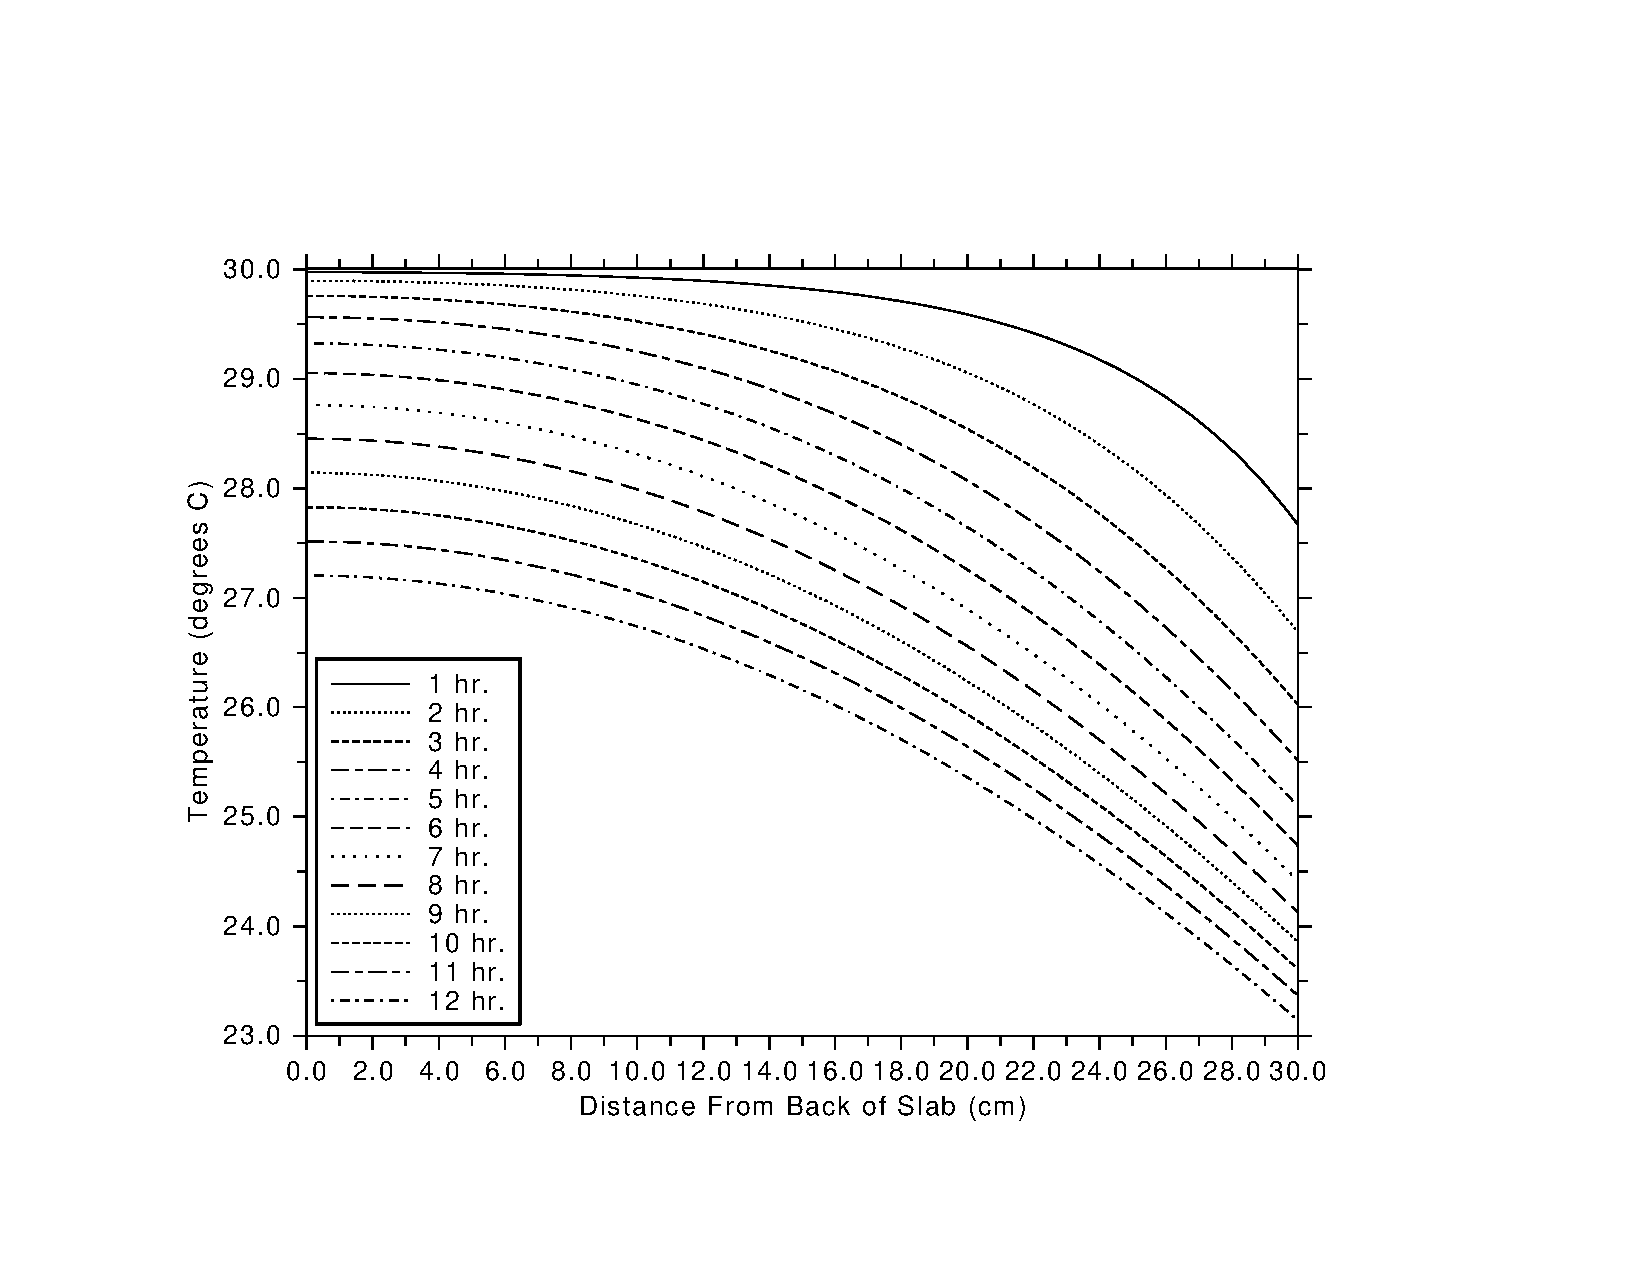
\includegraphics{dislin.pdf}}\caption{Predicted temperature of concrete slab.}
  \end{center}
\end{figure}

\newpage
\begin{table}[h]
\caption{Surface of wall temperature drop.}
\begin{center}
\begin{tabular}{|c|c|}
\hline {\bf Time (hr)} & {\bf Wall Surface Temp. ($^\circ$C)}\\
\hline 1 & 27.68 \\
\hline 2 & 26.70 \\
\hline 3 & 26.03 \\
\hline 4 & 25.52 \\
\hline 5 & 25.10 \\
\hline 6 & 24.74 \\
\hline 7 & 24.42 \\
\hline 8 & 24.13 \\
\hline 9 & 23.86 \\
\hline 10 & 23.61 \\
\hline 11 & 23.38 \\
\hline 12 & 23.15\\
\hline
\end{tabular}
\end{center}
\end{table}





The sensitivity analysis reveals how the temperature varies when
individual parameters are varied (Table 2). temperature is most
sensitive to decreases in $c$, the specific heat of concrete.  Since
$c$ effects heat flows through the slab, this finding is reasonable.
Varying $\rho$ has an identical effect on the model results (Table
3).

\begin{table}[!h]
\caption{Surface of wall temperature drop.}
\begin{center}
\begin{tabular}{|c|c|c|}
\hline {\bf Property}&{\bf Parameter} & {\bf Units}\\
\hline Conductivity &$h$ & $\frac{cal}{sec\cdot cm\cdot ^\circ C}$ \\
\hline Specific Heat &$c$ & $\frac{cal}{g\cdot ^\circ C}$ \\
\hline Density& $\rho$ &$\frac{g}{cm^3}$\\
\hline Heat Transfer Coefficient&$k$ & $\frac{cal}{sec\cdot cm^2\cdot ^\circ C}$\\
\hline
\end{tabular}
\end{center}
\end{table}

\begin{table}[!h]
\begin{center}
\caption{Parameters associated with determining wall temp.}
% Table generated by Excel2LaTeX from sheet 'AcrD227'
\begin{tabular}{|r|r|l|l|l|l|l|l|l|}
\hline
{\bf Run \#} & {\bf Variable} & {\bf Value}  & {\bf \% Varied} & {\bf New Value}    & {\bf Wall Temp.}  &{\bf Variation}\\
\hline
         1   &       $h$      &     0.0041338&       -10\%     & 3.72$\times10^{-3}$ &22.98              &0.69\%   \\
         2   &                &     0.0041338&        10\%     & 4.55$\times10^{-3}$ &23.29              &0.65\%   \\
\hline
         3   &     $c$        &      0.2     &       -10\%     &0.18                &22.86              &1.21\%   \\
         4   &                &    0.2       &        10\%     &0.22                &23.39              &1.08\%   \\
\hline
         5   &    $\rho$      &   2.24       &       -10\%     &2.016               &22.86              &1.21\%   \\
         6   &                &    2.24      &        10\%     &2.464               &23.89              &1.08\%   \\
\hline
         5   &    $k$         &   0.00013136 &       -10\%     &1.18$\times10^{-4}$  &23.57              &1.86\%   \\
         6   &                &  0.00013136  &        10\%     &1.44$\times10^{-4}$  &22.75              &1.69\%   \\
\hline
\end{tabular}
\end{center}
\end{table}

%\break\clearpage\pagebreak
\newpage
\section{Conclusion}
The following can be concluded from the analysis:
\begin{itemize}
\item{The surface of the wall loses heat quicker than any other part.}
\item{After 12 hours the surface of the wall is 23.14$^\circ$ C}
\item{The model is most sensitive to increases in $c$ and$\rho$.}
\item{The model is least sensitive to changes in $h$.}
\item{With the currently proposed conditions rate the wall is economically feasible.}
\end{itemize}

\section{References}
\noindent Finney,Brad. PDE Lab 2 handout, Humboldt State University,
Fall 2006.

\appendix
\newcommand{\appsection}[1]{\let\oldthesection\thesection
  \renewcommand{\thesection}{Appendix \oldthesection}
  \section{#1}\let\thesection\oldthesection}
\appsection{\\~Source Code} \label{sec:source}
\begin{singlespacing}
\begin{small}
\begin{Verbatim}[frame=single]
program pde2
  use dislin
  implicit none
  double precision,dimension(:),allocatable::a,b,c,d,x,t
  double precision::tstep,xstep,tini,phi,th,k,thk,ccon,p,h,Ts,time
  double precision::xa,xe,xor,xastep,ya,ye,yor,ystep
  integer::nxgrd,ntgrd,i,j
  character(len=6)::legendstring

  !Variable list

  interface
    subroutine tomas(a,b,c,d,x,neq)
      double precision,dimension(:),intent(out)::x
      double precision,dimension(:),intent(in)::a,b,c,d
      integer,intent(in)::neq
    end subroutine
  end interface


  open(11,file="prm.dat")
  open(12,file="heat.out")
  read(11,*)ntgrd,nxgrd,tini,thk,k,ccon,p,h,Ts,time
  write(*,*)nxgrd

  tstep=time/dble(ntgrd)
  write(*,*)tstep
  xstep=thk/nxgrd
  phi=(k*tstep)/(ccon*p*xstep**2)
  th=(h*tstep)/(ccon*p*xstep)

  allocate(a(nxgrd),b(nxgrd),c(nxgrd),d(nxgrd),x(nxgrd),t(nxgrd))
  write(*,*)"here"
  d(1:nxgrd-1)=30d0
  write(12,"(100f10.5)")(d(j),j=1,nxgrd)
  d(nxgrd)=30d0+2d0*th*Ts
  a(1)=0
  a(2:nxgrd-1)=-phi
  a(nxgrd)=-2d0*phi
  b(1:nxgrd-1)=1+2d0*phi
  b(nxgrd)=1d0+2d0*phi+2d0*th
  c(1)=-2d0*phi
  c(2:nxgrd-1)=-phi
  c(nxgrd)=0

  t(1)=0d0
  do i=2,nxgrd
    t(i)=t(i-1)+xstep
  end do

  xa=0d0 ! xa is the lower limit of the x-axis.
  xe=30d0 ! xe is the upper limit of the x-axis.
  xor=0 ! xor is the first x-axis label.
  xastep=2d0 ! xstep is the step between x-axis labels.
  ya=23d0 ! ya is the lower limit of the y-axis.
  ye=30.01d0 ! ye is the upper limit of the y-axis.
  yor=23d0 ! yor is the first y-axis label.
  ystep=1d0 ! ystep is the step between y-axis labels.
  !Plot data using DISLIN
  call metafl("xwin") ! or "PS", "EPS", "PDF", "WMF" "BMP"
  call setpag("USAL") !"USAL" is US size A landscape, "USAP" is portrait
  call scrmod("REVERS") !sets black on white background
  call disini() !Initialize dislin
  call complx ! Sets the font
  call name("Distance From Back of Slab (cm)","X") ! Set label for x-axis
  call name("Temperature (degrees C)","Y") ! Set label for y-axis
  !call titlin("Phosphorus Concentrations",1) ! Set 1st line of plot title
  call psfont("Helvetica")
  call graf (xa, xe, xor, xastep, ya, ye, yor, ystep) ! sets up axis
  call title ! Actually draw the title in over the axis
  !call grid(1,2)
  call legini(legendstring,12,8) ! Store 2 lines of legend text, max20 characters/line
  !CALL LEGPOS(2405,500) !defines a global position for the legend where NX and NY are the
                  !plot coordinates of the upper left corner. After a call to LEGPOS,
                  !the second parameter in LEGEND will be ignored.
  call FRAME(3)
  call legtit("") ! set legend title (default="legend")
  call leglin(legendstring,"1 hr.",1) ! Specify the legend text for curve 1
  call leglin(legendstring,"2 hr.",2)
  call leglin(legendstring,"3 hr.",3)
  call leglin(legendstring,"4 hr.",4)
  call leglin(legendstring,"5 hr.",5)
  call leglin(legendstring,"6 hr.",6)
  call leglin(legendstring,"7 hr.",7)
  call leglin(legendstring,"8 hr.",8)
  call leglin(legendstring,"9 hr.",9)
  call leglin(legendstring,"10 hr.",10)
  call leglin(legendstring,"11 hr.",11)
  call leglin(legendstring,"12 hr.",12)

  do i=1,ntgrd
    call tomas(a,b,c,d,x,nxgrd)
    write(12,"(100f10.5)")(x(j),j=1,nxgrd)
    write(12,*)""
    call curve(t,x,nxgrd) ! draw the x-y curve
    if(i>=8)then
      call lintyp(i-7) ! Change the line style (values are from 1 to 7)
    else
      call lintyp(i)
    end if
    d=x
    d(nxgrd)=x(nxgrd)+2d0*th*Ts
  end do

  call legend(legendstring,5) ! draw legend in 7 (upper right inside axis)
  !draw legend in location 1-8. 1-4=page corner, 5-8=axis corner,1 and 5=lowerleft
  call disfin ! finish off the plot

  rewind(12)
  rewind(11)
  stop
end program pde2


subroutine tomas(a,b,c,d,x,neq)
  implicit none
  double precision,dimension(:),intent(out)::x
  double precision,dimension(:),intent(in)::a,b,c,d
  integer,intent(in)::neq
  double precision,dimension(neq)::e,f
  integer::i,j

  e(1)=d(1)/b(1)
  f(1)=c(1)/b(1)

  do i=2,neq
    e(i)=(d(i)-a(i)*e(i-1))/(b(i)-a(i)*f(i-1))
    f(i)=c(i)/(b(i)-a(i)*f(i-1))
  end do

  x(neq)=e(neq)

  do i=neq-1,1,-1
    x(i)=e(i)-f(i)*x(i+1)
  end do

end subroutine

\end{Verbatim}
\end{small}
\end{singlespacing}
\noindent This was typeset with \LaTeX
\end{document}
